\documentclass[10pt]{beamer}\usepackage[]{graphicx}\usepackage[]{color}
%% maxwidth is the original width if it is less than linewidth
%% otherwise use linewidth (to make sure the graphics do not exceed the margin)
\makeatletter
\def\maxwidth{ %
  \ifdim\Gin@nat@width>\linewidth
    \linewidth
  \else
    \Gin@nat@width
  \fi
}
\makeatother

\definecolor{fgcolor}{rgb}{0.345, 0.345, 0.345}
\newcommand{\hlnum}[1]{\textcolor[rgb]{0.686,0.059,0.569}{#1}}%
\newcommand{\hlstr}[1]{\textcolor[rgb]{0.192,0.494,0.8}{#1}}%
\newcommand{\hlcom}[1]{\textcolor[rgb]{0.678,0.584,0.686}{\textit{#1}}}%
\newcommand{\hlopt}[1]{\textcolor[rgb]{0,0,0}{#1}}%
\newcommand{\hlstd}[1]{\textcolor[rgb]{0.345,0.345,0.345}{#1}}%
\newcommand{\hlkwa}[1]{\textcolor[rgb]{0.161,0.373,0.58}{\textbf{#1}}}%
\newcommand{\hlkwb}[1]{\textcolor[rgb]{0.69,0.353,0.396}{#1}}%
\newcommand{\hlkwc}[1]{\textcolor[rgb]{0.333,0.667,0.333}{#1}}%
\newcommand{\hlkwd}[1]{\textcolor[rgb]{0.737,0.353,0.396}{\textbf{#1}}}%

\usepackage{framed}
\makeatletter
\newenvironment{kframe}{%
 \def\at@end@of@kframe{}%
 \ifinner\ifhmode%
  \def\at@end@of@kframe{\end{minipage}}%
  \begin{minipage}{\columnwidth}%
 \fi\fi%
 \def\FrameCommand##1{\hskip\@totalleftmargin \hskip-\fboxsep
 \colorbox{shadecolor}{##1}\hskip-\fboxsep
     % There is no \\@totalrightmargin, so:
     \hskip-\linewidth \hskip-\@totalleftmargin \hskip\columnwidth}%
 \MakeFramed {\advance\hsize-\width
   \@totalleftmargin\z@ \linewidth\hsize
   \@setminipage}}%
 {\par\unskip\endMakeFramed%
 \at@end@of@kframe}
\makeatother

\definecolor{shadecolor}{rgb}{.97, .97, .97}
\definecolor{messagecolor}{rgb}{0, 0, 0}
\definecolor{warningcolor}{rgb}{1, 0, 1}
\definecolor{errorcolor}{rgb}{1, 0, 0}
\newenvironment{knitrout}{}{} % an empty environment to be redefined in TeX

\usepackage{alltt}
%\usepackage[orientation=portrait,size=A4]{beamerposter}
\usetheme{ttu}
%%%%%% End Use for handouts
\usepackage{graphics,graphicx,epsf,epsfig,pstricks}
\usepackage{soul}
%\setulcolor{ucsbyellow}
\setulcolor{ttured}
%\usepackage{pgf}
\usepackage{textpos}
\usepackage{pdfsync}
\usepackage{bm,bbm}
\usepackage{amsmath}
\usepackage{sidecap}
\usepackage{pgf}

\usepackage[sc]{mathpazo}
\usepackage[T1]{fontenc}
\usepackage{geometry}
%\geometry{verbose,tmargin=2.5cm,bmargin=2.5cm,lmargin=2.5cm,rmargin=2.5cm}
\usepackage{url}
\usepackage{breakurl}



%%%%%% Other possible themes
%\useoutertheme{infolines}
% items enclosed in square brackets are optional; explanation below
\title[GIST4302]{{\Large GIST 4302: Spatial Analysis and Modeling }}
\subtitle[Point Pattern Analysis]{\small Point Pattern Analysis}
\author[Guofeng Cao]{Guofeng Cao\\ [1.0ex]
\scriptsize{www.cigi.uiuc.edu/guofeng}}
%%% INSTITUTE
\institute[Texas Tech]{
\includegraphics[height=1.5cm]{TTU-seal-color.pdf}\\[1.0ex]
  Department of Geosciences\\ [0.5ex]
  Texas Tech University\\[1.5ex]
 \texttt{guofeng.cao@ttu.edu} \\[2ex]
}
%
\date[TTU]{Fall 2013}

%%% LOGOS
%\logo{\vspace{7.65cm}\includegraphics[width=1.5cm]{logoUCSB.pdf}}
%\logo{\vspace{7.65cm} \includegraphics[width=0.8cm]{TTU-seal-color.pdf}}
\logo{\pgfputat{\pgfxy(-12.1,7.65)}{\pgfbox[center,base]{\includegraphics[width=0.8cm]{TTU-seal-color.pdf}}}}
% For theme Malmoe, logo is inserted at lower right corner,
% \vspace{+} moves logo upwards...

% Set color of equations to blue
%%%%%%%%%%%%%%%%%%%%%%%%%%%%%%%%%%%%%%%%%%%%%%%%%%%%%%%%%%%%%%%%%%%%
%\everymath{\color{blue}}        % For inline equations
\everymath{\color{ttured}}        % For inline equations
%\everydisplay{\color{blue}}     % For displayed equations
\everydisplay{\color{ttured}}     % For displayed equations
%%%%%%%%%%%%%%%%%%%%%%%%%%%%%%%%%%%%%%%%%%%%%%%%%%%%%%%%%%%%%%%%%%%%
% Set symbol shortcuts
%%%%%%%%%%%%%%%%%%%%%%%%%%%%%%%%%%%%%%%%%%%%%%%%%%%%%%%%%%%%%%%%%%%%
\newcommand{\vecth}{\boldsymbol{\theta}}
\newcommand{\matS}{\boldsymbol{\Sigma}}
\newcommand{\vecs}{\boldsymbol{\sigma}}
\newcommand{\vecss}{\boldsymbol{s}}
\newcommand{\vecr}{\boldsymbol{\rho}}
\newcommand{\vecl}{\boldsymbol{\lambda}}
\newcommand{\matPhi}{\boldsymbol{\Phi}}
\newcommand{\vecb}{\boldsymbol{\beta}}
\newcommand{\vecm}{\boldsymbol{\mu}}
\newcommand{\matO}{\boldsymbol{\Omega}}
\newcommand{\Var}{\mathbb{V}ar}
\newcommand{\Cov}{\mathbb{C}ov}
\newcommand{\Exp}{\mathbb{E}}
\newcommand{\Prob}{\mathbb{P}ropb}
\newcommand{\vy}{\mathbf{\mathbbmtt{y}}}
\newcommand{\loc}{\mathbf{x}}
\newcommand{\vech}{\mathbf{h}}
\newcommand{\loch}{\mathbf{h}}

\newcommand{\vecx}{\boldsymbol{x}}
\newcommand{\vecX}{\boldsymbol{X}}
\newcommand{\veczero}{\boldsymbol{0}}
\newcommand{\vecu}{\boldsymbol{u}}
\newcommand{\vecw}{\boldsymbol{w}}
\newcommand{\vecW}{\boldsymbol{W}}
\newcommand{\vecK}{\boldsymbol{K}}
\newcommand{\vecI}{\boldsymbol{I}}
\newcommand{\vecc}{\boldsymbol{c}}
\newcommand{\vecbeta}{\boldsymbol{\beta}}
\newcommand{\vectheta}{\boldsymbol{\theta}}
\newcommand{\vecmu}{\boldsymbol{\mu}}
\newcommand{\vecpi}{\boldsymbol{\pi}}
\newcommand{\vecepsilon}{\boldsymbol{\varepsilon}}
\newcommand{\argmax}{\operatornamewithlimits{argmax}}
\newtheorem{proposition}{Proposition: Transiogram and Perimeter-to-Area Ratio}
\newtheorem{proposition2}{Proposition: Validity of Transiogram Models}
%
\newcommand{\abs}[1]{\lvert#1\rvert}
\newcommand{\norm}[1]{\lVert#1\rVert}
%%%%%%%%%%%%%%%%%%%%%%%%%%%%%%%%%%%%%%%%%%%%%%%%%%%%%%%%%%%%%%%%%%%%
% Set list & environment shortcuts
%%%%%%%%%%%%%%%%%%%%%%%%%%%%%%%%%%%%%%%%%%%%%%%%%%%%%%%%%%%%%%%%%%%%
\newcommand{\bcenter}{\begin{center}}
\newcommand{\ecenter}{\end{center}}
\newcommand{\bfigure}{\begin{figure}}
\newcommand{\efigure}{\end{figure}}
\newcommand{\bitemize}{\begin{itemize}}
\newcommand{\eitemize}{\end{itemize}}
\newcommand{\benumer}{\begin{enumerate}}
\newcommand{\eenumer}{\end{enumerate}}
%\newcommand{\bframe}{\begin{frame}}
%\newcommand{\eframe}{\end{frame}}
\newcommand{\bblock}{\begin{block}}
\newcommand{\eblock}{\end{block}}

%\AtBeginSubsection[]
%{
%   \begin{frame}
%       \frametitle{Outline}
%       \tableofcontents[currentsection,currentsubsection]
%   \end{frame}
%}
%%%%%%%%%%%%%%%%%%%%%%%%%%%%%%%%%%%%%%%%%%%%%%%%%%%%%%%%%%%%%%%%%%%%
\IfFileExists{upquote.sty}{\usepackage{upquote}}{}
\begin{document}




%%%%%%%%%%%%%% The titlepage frame %%%%%%%%%%%%%%%%%%%%%%%%%%%%%%%%%%
\begin{frame}[plain]
  \titlepage
\end{frame}
%%%%%%%%%%%%%%%%%%%%%%%%%%%%%%%%%%%%%%%%%%%%%%%%%%%%%%%%%%%%%%%%%%%%%
%\begin{frame}%[squeeze]
%\frametitle{Outline}
%\tableofcontents%[pausesections]
%\end{frame}
%%%%%%%%%%%%%%%%%%%%%%%%%%%%%%%%%%%%%%%%%%%%%%%%%%%%%%%%%%%%%%%%%%%%%
%%%%%%%%%%%%%%%%%%%%%%%%%%%%%%%%%%%%%%%%%%%%%%%%%%%%%%%%%%%%%%%%%%%%%
\begin{frame}
\frametitle{Spatial Point Patterns}
\bblock{Characteristics:}
\begin{itemize}
	\item set of $n$ point locations with recorded ``events'', e.g., locations of trees, disease or crime incidents
		$S=\{\vecss_1,\ldots,\vecss_i,\ldots, \vecss_n\}$
	\item point locations correspond to all possible events or to subsets of them
\item attribute values also possible at same locations, e.g., tree diameter, magnitude of earthquakes ({\it marked point pattern}) $W=\{w_1,\ldots,w_i,\ldots, w_n\}$
\end{itemize}
\eblock
\bblock{Analysis objectives:}
\begin{itemize}
\item detect spatial clustering or repulsion, as opposed to complete randomness, of event locations (in space and time)
\item if clustering detected, investigate possible relations with nearby ``sources''
\end{itemize}
\eblock
\end{frame}

%%%%%%%%%%%%%%%%%%%%%%%%%%%%%%%%%%%%%%%%%%%%%%%%%%%%%%%%%%%%%%%%%%%%%%
\begin{frame}
\frametitle{Spatial Point Patterns}
\bblock{Further issues:}
\begin{itemize}
\item analysis of point patterns over large areas should take into account distance distortions due to map projections
\item boundaries of study area should not be arbitrary
\item analysis of sampled point patterns can be misleading
\item one-to-one correspondence between objects in study area and events in pattern 
\end{itemize}
\eblock

\end{frame}
%%%%%%%%%%%%%%%%%%%%%%%%%%%%%%%%%%%%%%%%%%%%%%%%%%%%%%%%%%%%%%%%%%%%

%%%%%%%%%%%%%%%%%%%%%%%%%%%%%%%%%%%%%%%%%%%%%%%%%%%%%%%%%%%%%%%%%%%%%%
\begin{frame}
\frametitle{Simple Descriptive Statistics}
\bblock{Mean center of a point pattern:}
\begin{itemize}
\item point with coordinates $\bar{s} = (\bar{x}, \bar{y})$:
\begin{equation*}
\bar{x}=\frac{\sum_{i=1}^{n} w_ix_i}{\sum_{i=1}^nw_i} \qquad {and} \qquad \bar{y}=\frac{\sum_{i=1}^{n} w_iy_i}{\sum_{i=1}^nw_i}
\end{equation*}
\item center of point pattern, or point with average $x$ and $y$-coordinates
\end{itemize}
\eblock

\vspace{-0.2cm}
\bblock{Median center of a point pattern:}
\bitemize
\item \underline{\it both} of the following two centers are called \underline{\it median centers}, although they are essentially different (confusing!)
\bitemize
\item the intersection between the median of the $x$ and the $y$ coordinates
\item {\it center for minimum distance:} $\vecss_c\in\{\vecss_1, \ldots, \vecss_n\}  s.t.  min \sum\limits_{i=1}^{n}|\vecss_i-\vecss_c|$
\eitemize
\item the first type of {\it median center} is not unique, and there is \underline{no} closed form for the second type
\item $p$-median problem (a tppical problem in spatial optimization ): {\scriptsize the problem of locating $p$ ``facilities'' relative to a set of ``customers'' such that the sum of the shortest demand weighted distance between ``customers'' and ``facilities'' is minimized}
\eitemize
\eblock


\end{frame}
%%%%%%%%%%%%%%%%%%%%%%%%%%%%%%%%%%%%%%%%%%%%%%%%%%%%%%%%%%%%%%%%%%%%%%%
%\begin{frame}
%\frametitle{Simple Descriptive Statistics}
%\bblock{Example of standard distance:}
%\bitemize
%\item Example: 
%
%\underline{\small \it mean center:} $\bar{s}=\{610941.3,4830837\}$ 
%
%\underline{\small \it standard distance:} $d_{std}=8117.952$
%
%<<sdd, fig.width=4, fig.height=4, out.width='.6\\linewidth', echo=FALSE, results='hide', warning=FALSE>>=
%## two plots side by side (option fig.show='hold')
%library(aspace)
%plot_sdd(plotnew=TRUE, plothv=FALSE, plotweightedpts=FALSE, plotpoints=TRUE, plotcentre=TRUE, titletxt="SDD", xaxis="Easting (m)", 
%yaxis="Northing (m)", sdd.col='black', centre.col='red')
%@
%
%\eitemize
%\eblock
%
%
%
%\end{frame}
%%%%%%%%%%%%%%%%%%%%%%%%%%%%%%%%%%%%%%%%%%%%%%%%%%%%%%%%%%%%%%%%%%%%

%%%%%%%%%%%%%%%%%%%%%%%%%%%%%%%%%%%%%%%%%%%%%%%%%%%%%%%%%%%%%%%%%%%%%%
\begin{frame}
\frametitle{Simple Descriptive Statistics}
\bblock{Changes of population center (year 1790-2000):}
\bcenter
\scalebox{0.4}{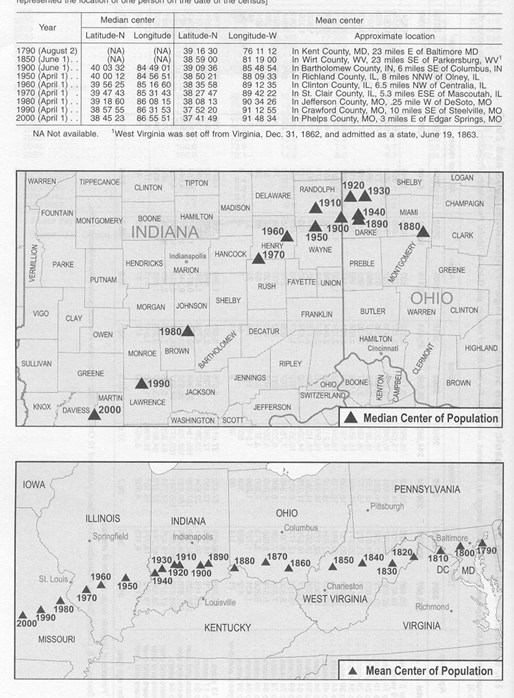
\includegraphics{pop-mean.png}}
\ecenter
\eblock
\end{frame}
%%%%%%%%%%%%%%%%%%%%%%%%%%%%%%%%%%%%%%%%%%%%%%%%%%%%%%%%%%%%%%%%%%%%


%%%%%%%%%%%%%%%%%%%%%%%%%%%%%%%%%%%%%%%%%%%%%%%%%%%%%%%%%%%%%%%%%%%%%%
\begin{frame}
\frametitle{Descriptive Statistics}

\bblock{Standard distance of a point pattern:}
\begin{itemize}
\item average squared deviations of $x$ and $y$ coordinates from their respective mean:
\begin{equation*}
d_{std} = \sqrt{\frac{\sum_{i=1}^{n}(x_i-\bar{x})^2+\sum_{i=1}^{n}(y_i-\bar{y})^2}{n-2}}
\end{equation*}

\item related to standard deviation of coordinates, a summary circle (centered at $\bar{s}$ with radius $d_{std}$) of a point pattern
\end{itemize}
\eblock

\bblock{Standard devitional ellipse:}
\bitemize
\item Taking directional effects into account for \underline{\it anisotropy} cases
\item Please refer to Levine and Associates, 2004 for calculations
\eitemize
\eblock

\end{frame}
%%%%%%%%%%%%%%%%%%%%%%%%%%%%%%%%%%%%%%%%%%%%%%%%%%%%%%%%%%%%%%%%%%%%%%

%%%%%%%%%%%%%%%%%%%%%%%%%%%%%%%%%%%%%%%%%%%%%%%%%%%%%%%%%%%%%%%%%%%%%%
\begin{frame}
\frametitle{Descriptive Statistics}

\bblock{Examples:}

\begin{knitrout}
\definecolor{shadecolor}{rgb}{0.969, 0.969, 0.969}\color{fgcolor}

{\centering \includegraphics[width=.5\linewidth]{figure/point-sde1} 
\includegraphics[width=.5\linewidth]{figure/point-sde2} 

}



\end{knitrout}

\eblock

\bblock{Remarks:}
\bitemize
\item indicates overall shape and center of point pattern
\item \underline{\it do not suffice to fully specify a spatial point pattern}
\eitemize
\eblock
\end{frame}
%%%%%%%%%%%%%%%%%%%%%%%%%%%%%%%%%%%%%%%%%%%%%%%%%%%%%%%%%%%%%%%%%%%%%%


\begin{frame}
\frametitle{Point Pattern Analysis Methods}
\bblock{1st order (i.e., intensity): absolute location of events on map:}
\bitemize
\item Quadrat methods 
\item Density Estimation (KDE)
\item Moran's I and Geary's C
\eitemize
\eblock

\bblock{2nd order (i.e., interactions): interaction of events:}
\bitemize
\item Nearest neighbor distance
\item Distance functions G, K, F, L 
\item Getis-Ord Gi* and Anselin local Moran's I 
\eitemize
\eblock
\end{frame}
%%%%%%%%%%%%%%%%%%%%%%%%%%%%%%%%%%%%%%%%%%%%%%%%%%%%%%%%%%%%%%%%%%%%

%%%%%%%%%%%%%%%%%%%%%%%%%%%%%%%%%%%%%%%%%%%%%%%%%%%%%%%%%%%%%%%%%%%%%%
\begin{frame}
\frametitle{Quadrat methods}
Consider a point pattern with $n$ events within a study region $A$ of area $|A|$

\bblock{Global intensity:}
\[
\hat{\lambda} = \frac{n}{|A|}=\frac{\# \mbox{of events within} A}{|A|}
\]
\eblock
\bblock{Local intensity via quadrats}
\benumer
\item partition $A$ into $L$ sub-regions ${A_l, l = 1, \ldots, L}$ of equal area $|A_l|$ (also called quadrats)
\item count number of events $n(A_l)$ in each sub-region $A_l$
\item convert sample counts into estimated intensity rates as:
\[
\hat{\lambda}(A_l) = \frac{n(A_l)}{|A_l|}
\]
\eenumer
\eblock
\end{frame}
%%%%%%%%%%%%%%%%%%%%%%%%%%%%%%%%%%%%%%%%%%%%%%%%%%%%%%%%%%%%%%%%%%%%

%%%%%%%%%%%%%%%%%%%%%%%%%%%%%%%%%%%%%%%%%%%%%%%%%%%%%%%%%%%%%%%
\begin{frame}
\frametitle{Quadrat methods}
%\vspace{-1cm}
\begin{knitrout}
\definecolor{shadecolor}{rgb}{0.969, 0.969, 0.969}\color{fgcolor}

{\centering \includegraphics[width=.6\linewidth]{figure/point-quad1} 

}



\end{knitrout}

\vspace{-1.5cm}
\bitemize
\item estimated rates $\hat{\lambda}(A_l)$ over set of quadrats 
\item reveal large-scale patterns in intensity variation over $A$ 
\item larger quadrats yield smoother intensity maps; smaller quadrats yield `spiky' intensity maps
\item size, origin, and shape of quadrats is critical (recall: {\it $MAUP$})
\item \underline{\it only first-order effects are captured}
\eitemize
\end{frame}
%%%%%%%%%%%%%%%%%%%%%%%%%%%%%%%%%%%%%%%%%%%%%%%%%%%%%%%%%%%%%%%%%%%%

%%%%%%%%%%%%%%%%%%%%%%%%%%%%%%%%%%%%%%%%%%%%%%%%%%%%%%%%%%%%%%%
\begin{frame}
\frametitle{Dependence of intensity on a covariate (Inhomogeneous cases)}
%\vspace{-1cm}
\begin{knitrout}
\definecolor{shadecolor}{rgb}{0.969, 0.969, 0.969}\color{fgcolor}

{\centering \includegraphics[width=.8\linewidth]{figure/point-covariate} 

}



\end{knitrout}


\end{frame}
%%%%%%%%%%%%%%%%%%%%%%%%%%%%%%%%%%%%%%%%%%%%%%%%%%%%%%%%%%%%%%%%%%%%

%%%%%%%%%%%%%%%%%%%%%%%%%%%%%%%%%%%%%%%%%%%%%%%%%%%%%%%%%%%%%%%
\begin{frame}
\frametitle{Kernel Density Estimation}
\bblock{Procedure of Kernel Density Estimation (KDE)}
\benumer
\item define a kernel $K(\vecss;r)$ of radius (or bandwidth) $r$ centered at any arbitrary location $\vecss$
\item estimate local intensity at $\vecss$ as:
\[
\hat{\lambda}(\vecss) = \frac{1}{n}\sum\limits_{i=1}^{n}K(\vecss_i-\vecss;r)
\]
\item repeat estimation for all points s in the study region to create a density map
\eenumer

\bfigure
\scalebox{0.2}{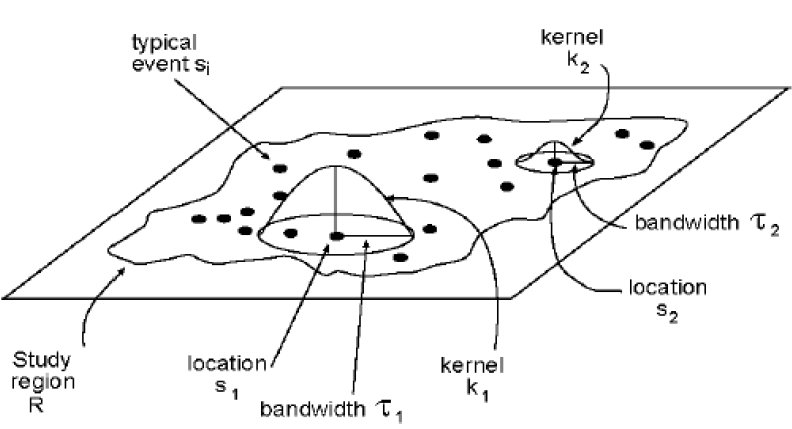
\includegraphics{kde.png}}
\efigure

\eblock


\end{frame}
%%%%%%%%%%%%%%%%%%%%%%%%%%%%%%%%%%%%%%%%%%%%%%%%%%%%%%%%%%%%%%%%%%%%

%%%%%%%%%%%%%%%%%%%%%%%%%%%%%%%%%%%%%%%%%%%%%%%%%%%%%%%%%%%%%%%
\begin{frame}
\frametitle{Kernel Density Estimation}
\bblock{Example for the previous dataset:}
\begin{knitrout}
\definecolor{shadecolor}{rgb}{0.969, 0.969, 0.969}\color{fgcolor}

{\centering \includegraphics[width=.5\linewidth]{figure/point-kde1} 
\includegraphics[width=.5\linewidth]{figure/point-kde2} 

}



\end{knitrout}

\eblock

\end{frame}
%%%%%%%%%%%%%%%%%%%%%%%%%%%%%%%%%%%%%%%%%%%%%%%%%%%%%%%%%%%%%%%%%%%%


%%%%%%%%%%%%%%%%%%%%%%%%%%%%%%%%%%%%%%%%%%%%%%%%%%%%%%%%%%%%%%%
\begin{frame}
\frametitle{Kernel Density Estimation}

\bblock{Example with 2km bandwidth}
\bfigure
\scalebox{0.4}{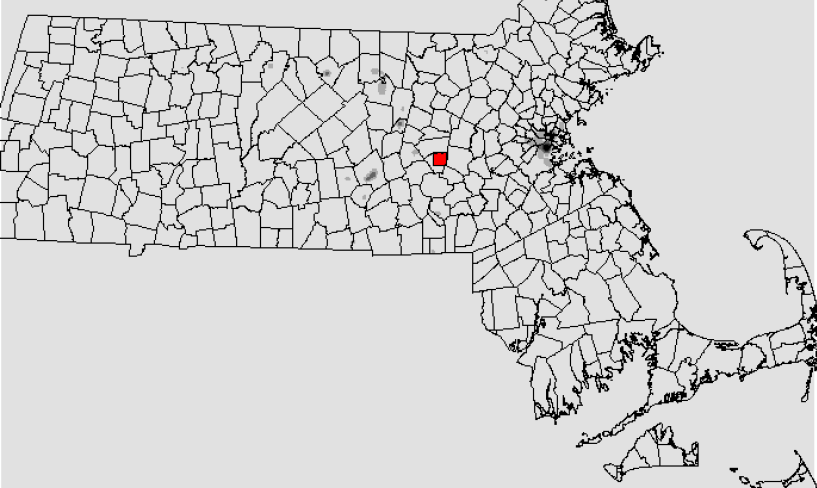
\includegraphics{kde1.png}}
\efigure
\eblock

\end{frame}

%%%%%%%%%%%%%%%%%%%%%%%%%%%%%%%%%%%%%%%%%%%%%%%%%%%%%%%%%%%%%%%%%%%%

%%%%%%%%%%%%%%%%%%%%%%%%%%%%%%%%%%%%%%%%%%%%%%%%%%%%%%%%%%%%%%%
\begin{frame}
\frametitle{Kernel Density Estimation}

\bblock{Example with 10km bandwidth}
\bfigure
\scalebox{0.4}{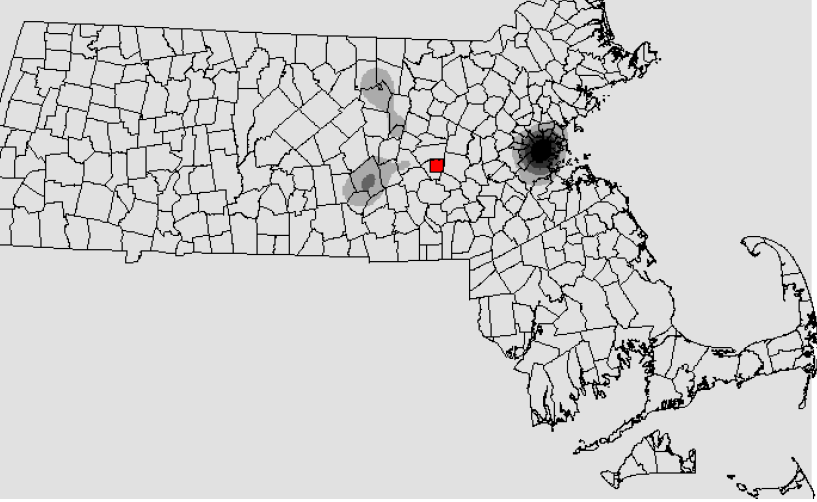
\includegraphics{kde2.png}}
\efigure
\eblock

\end{frame}
%%%%%%%%%%%%%%%%%%%%%%%%%%%% %%%%%%%%%%%%%%%%%%%%%%%%%%%%

\begin{frame}
\frametitle{Kernel Density Estimation}

\bblock{Example with 40km bandwidth}
\bfigure
\scalebox{0.4}{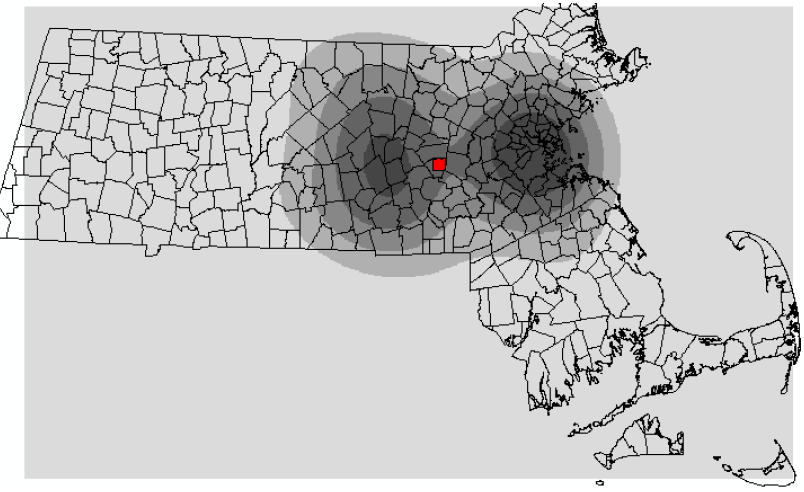
\includegraphics{kde3.png}}
\efigure
\eblock

\end{frame}

%%%%%%%%%%%%%%%%%%%%%%%%%%%%%%%%%%%%%%%%%%%%%%%%%%%%%%%%%%%%%%%

%%%%%%%%%%%%%%%%%%%%%%%%%%%%%%%%%%%%%%%%%%%%%%%%%%%%%%%%%%%%%%%
\begin{frame}
\frametitle{Kernel Density Estimation}

\bblock{Comments}
\bitemize
\item Choice of kernel function is not critical (Diggle, 1985) 
\item Choice of bandwidth, or degree of smoothing critical: 
\bitemize
\item Small bandwidth $\rightarrow$ spiky results
\item Large bandwidth $\rightarrow$ loss of detail
\eitemize
\item Multi-scale analyses can use these bandwidth characteristics to investigate both broad trends and localized variation
\item How to choose bandwidth: choose the degree of smoothing subjectively, by eye, or by formula (Diggle) 
\item could define local bandwidth based on function of presence of events in neighborhood of $\vecss$ (i.e., adaptive kernel estimation)
\eitemize
\eblock

\end{frame}

%%%%%%%%%%%%%%%%%%%%%%%%%%%%%%%%%%%%%%%%%%%%%%%%%%%%%%%%%%%%%%%%%%%%

%%%%%%%%%%%%%%%%%%%%%%%%%%%%%%%%%%%%%%%%%%%%%%%%%%%%%%%%%%%%%%%
\begin{frame}
\frametitle{Distance-based Descriptors of Point Patterns}

\bblock{Distances}
\bitemize
\item Accessing second order effects
\bitemize
\item Event-to-event distance: distance $d_{ij}$ between event at arbitrary location $s_i$ and another
event at another arbitrary location $s_j$:
{\scriptsize \[
d_{ij} = \sqrt{(x_i - x_j)^2 + (y_i-y_j)^2}
\]}

\item Point-to-event distance: distance $\tilde{d}_{pj}$ between a randomly chosen point at location $\tilde{s}_p$
and an event at location $s_j$:

{\scriptsize \[
\tilde{d}_{pj} = \sqrt{(\tilde{x}_p - x_j)^2 + (\tilde{y}_i-y_j)^2}
\]
}

\item Event-to-nearest-neighbour distance: distance $d_{min}(s_i)$ between an event at location $s_i$ and its
{\it nearest neighbor} event: 
{\scriptsize \[
d_{min}(s_i) = min\{d_{ij}, j \neq i, j = 1, \ldots,n\}
\]
}
\item Point-to-nearest-neighbour distance (i.e., {\it empty space distance}): distance $d_{min}(\tilde{s}_p)$ between a randomly chosen point at location
$\tilde{s}_p$ and its {\it nearest neighbor} event:

{\scriptsize \[
\tilde{d}_{min}(\tilde{s}_p) = min\{\tilde{d}_{pj}, j = 1, \ldots,n\}
\]}

\eitemize
\eitemize
\eblock
\end{frame}

%%%%%%%%%%%%%%%%%%%%%%%%%%%%%%%%%%%%%%%%%%%%%%%%%%%%%%%%%%%%%%%
\begin{frame}
\frametitle{Event-to-Nearest-Neighbor Distances}



{\centering \includegraphics[width=.4\linewidth]{figure/point-points} 

}





% latex table generated in R 3.0.1 by xtable 1.7-1 package
% Thu Sep 26 12:56:45 2013
\begin{table}[ht]
\centering
\begin{tabular}{rrrrrr}
  \hline
 & 1 & 2 & 3 & 4 & 5 \\ 
  \hline
1 & 0.00 & 11947.70 & 16042.65 & 3481.22 & 10742.98 \\ 
  2 & 11947.70 & 0.00 & 5126.79 & 15219.58 & 1599.07 \\ 
  3 & 16042.65 & 5126.79 & 0.00 & 19481.59 & 6720.59 \\ 
  4 & 3481.22 & 15219.58 & 19481.59 & 0.00 & 13913.70 \\ 
  5 & 10742.98 & 1599.07 & 6720.59 & 13913.70 & 0.00 \\ 
   \hline
\end{tabular}
\caption{Euclidean distance matrix} 
\end{table}


\end{frame}
%%%%%%%%%%%%%%%%%%%%%%%%%%%%%%%%%%%%%%%%%%%%%%%%%%%%%%%%%%%%%%%%%%%%

%%%%%%%%%%%%%%%%%%%%%%%%%%%%%%%%%%%%%%%%%%%%%%%%%%%%%%%%%%%%%%%
\begin{frame}
\frametitle{Event-to-Nearest-Neighbor Distances}

\bblock{Nearest neighour distances}
\begin{knitrout}
\definecolor{shadecolor}{rgb}{0.969, 0.969, 0.969}\color{fgcolor}

{\centering \includegraphics[width=.5\linewidth]{figure/point-nn} 

}



\end{knitrout}


\bitemize
\item Mean nearest neighbour distance: Average of all $d_{min}(s_i)$ values
\[
\bar{d}_{min} = \frac{1}{n}\sum\limits_{i=1}^{n}d_{min}(s_i)
\]
\eitemize


\eblock
\end{frame}
%%%%%%%%%%%%%%%%%%%%%%%%%%%%%%%%%%%%%%%%%%%%%%%%%%%%%%%%%%%%%%%

%%%%%%%%%%%%%%%%%%%%%%%%%%%%%%%%%%%%%%%%%%%%%%%%%%%%%%%%%%%%%%%
\begin{frame}
\frametitle{The G function}
\bblock{Definition}
\bitemize
\item nearest neighbour distance function, i.e.,  proportion of event-to-nearest-neighbor distances $d_{min}(s_i)$
no greater than given distance cutoff $d$, estimated as:
\[
\hat{G}(d) = \frac{\#\{d_{min}(s_i)<d, i = 1, \ldots, n\}}{n}
\]
 
\item alternative definition: cumulative distribution function
(CDF) of all $n$ event-to-nearest-neighbor distances; instead of computing average  $\bar{d}_{min}$ of $d_{min}$ values, compute their CDF
\item the G function provides information on event {\it proximity}
\item example for previous clustering point pattern:


{\centering \includegraphics[width=.3\linewidth]{figure/point-freq1} 
\includegraphics[width=.3\linewidth]{figure/point-freq2} 

}




\eitemize
\eblock
\end{frame}
%%%%%%%%%%%%%%%%%%%%%%%%%%%%%%%%%%%%%%%%%%%%%%%%%%%%%%%%%%%%%%%%%%%%end{frame}

%%%%%%%%%%%%%%%%%%%%%%%%%%%%%%%%%%%%%%%%%%%%%%%%%%%%%%%%%%%%%%%
\begin{frame}
\frametitle{Examples of G function}


{\centering \includegraphics[width=.5\linewidth]{figure/point-ghat1} 

}




\bblock{Expected plot: }
\bitemize
\item for clustered events, $\hat{G}(d)$ rises sharply at short distances, and
then levels off at larger $d$-values
\item for randomly-spaced events, $\hat{G}(d)$ rises gradually up to the distance
at which most events are spaced, and then increases sharply
\eitemize
\eblock
\end{frame}
%%%%%%%%%%%%%%%%%%%%%%%%%%%%%%%%%%%%%%%%%%%%%%%%%%%%%%%%%%%%%%%%%%%%end{frame}

%%%%%%%%%%%%%%%%%%%%%%%%%%%%%%%%%%%%%%%%%%%%%%%%%%%%%%%%%%%%%%%
\begin{frame}
\frametitle{The F function}
\bblock{Definition}
\bitemize
\item proportion of point-to-nearest-neighbor distances (i.e., {\it empty space distances}) $\tilde{d}_{min}(s_p)$
no greater than given distance cutoff $d$, estimated as:

\[
\hat{F}(d) = \frac{\#\{\tilde{d}_{min}(\tilde{s}_p)<d, p = 1, \ldots, m\}}{m}
\]
\item alternative definition: cumulative distribution function
(CDF) of all $m$ point-to-nearest-neighbor distances
\item the F function provides information on event proximity to voids
\item Examples for previous clustering point pattern:


{\centering \includegraphics[width=.3\linewidth]{figure/point-f1} 
\includegraphics[width=.3\linewidth]{figure/point-f2} 
\includegraphics[width=.3\linewidth]{figure/point-f3} 

}




\eitemize
\eblock
\end{frame}
%%%%%%%%%%%%%%%%%%%%%%%%%%%%%%%%%%%%%%%%%%%%%%%%%%%%%%%%%%%%%%%%%%%%end{frame}

%%%%%%%%%%%%%%%%%%%%%%%%%%%%%%%%%%%%%%%%%%%%%%%%%%%%%%%%%%%%%%%
\begin{frame}
\frametitle{Examples of F function}


{\centering \includegraphics[width=.5\linewidth]{figure/point-fhat1} 

}




\bblock{Expected plot: }
\bitemize
\item for clustered events, $\hat{F}(d)$ rises sharply at short distances, and
then levels off at larger $d$-values

\item for randomly-spaced events, $\hat{F}(d)$ rises rapidly up to the distance at
which most events are spaced, and then levels off (there are more
nearest neighbors at small distances from randomly placed points)
\eitemize
\eblock
\end{frame}
%%%%%%%%%%%%%%%%%%%%%%%%%%%%%%%%%%%%%%%%%%%%%%%%%%%%%%%%%%%%%%%%%%%%end{frame}

%%%%%%%%%%%%%%%%%%%%%%%%%%%%%%%%%%%%%%%%%%%%%%%%%%%%%%%%%%%%%%%
\begin{frame}
\frametitle{Comparing G and F functions}



{\centering \includegraphics[width=.5\linewidth]{figure/point-fhatghat} 

}




\bblock{Expected plot: }
\bitemize
\item for clustered events, $\hat{G}(d)$ rises faster
\item for randomly-spaced events, $\hat{F}(d)$ tends to be close to $\hat{G}(d)$  
 
\eitemize
\eblock
\end{frame}
%%%%%%%%%%%%%%%%%%%%%%%%%%%%%%%%%%%%%%%%%%%%%%%%%%%%%%%%%%%%%%%%%%%%end{frame}


%%%%%%%%%%%%%%%%%%%%%%%%%%%%%%%%%%%%%%%%%%%%%%%%%%%%%%%%%%%%%%%
\begin{frame}
\frametitle{The K function}
{\it \small Working with pair-wise distances\&looking beyond nearest neighours}
\bblock{Concept}
\benumer
\item construct set of concentric circles (of increasing radius $d$) around
each event
\item count number of events in each distance ``band''
\item cumulative number of events up to radius $d$ around all events
becomes the sample $K$ function $\hat{K}(d)$ 
\eenumer
\bfigure
\scalebox{0.2}{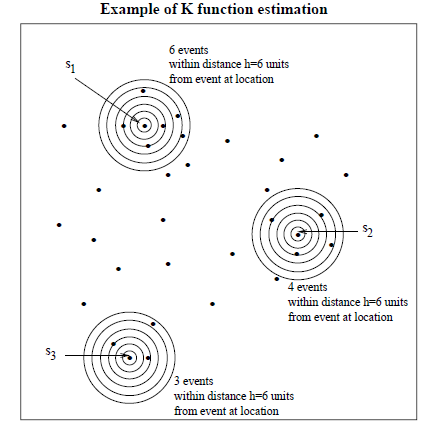
\includegraphics{k.png}}
\efigure

\eblock
\end{frame}
%%%%%%%%%%%%%%%%%%%%%%%%%%%%%%%%%%%%%%%%%%%%%%%%%%%%%%%%%%%%%%%%%%%%end{frame}

%%%%%%%%%%%%%%%%%%%%%%%%%%%%%%%%%%%%%%%%%%%%%%%%%%%%%%%%%%%%%%%
\begin{frame}
\frametitle{The K function}
{\it \small Working with pair-wise distances\&looking beyond nearest neighours}
\bitemize
\item Formal definition:
\begin{align*}
K(d) &= \frac{1}{\lambda}\frac{\# \{d_{ij}\leq d, i, j=1,\ldots, n\}}{n} \\
&=\frac{|A|}{n}\frac{\# \{d_{ij}\leq d, i, j=1,\ldots, n\}}{n} \\
&= |A|(\mbox{proportion of event-to-event distance} \leq d)
\end{align*}
\item In other words, the $\hat{K}(d)$ is the sample cumulative distribution
function (CDF) of all $n^2$ event-to-event distances, scaled by $|A|$
\eitemize
\end{frame}
%%%%%%%%%%%%%%%%%%%%%%%%%%%%%%%%%%%%%%%%%%%%%%%%%%%%%%%%%%%%%%%%%%%%

%%%%%%%%%%%%%%%%%%%%%%%%%%%%%%%%%%%%%%%%%%%%%%%%%%%%%%%%%%%%%%%
\begin{frame}
\frametitle{Examples of Event-to-Event Distance Histogram and CDFs}



{\centering \includegraphics[width=.8\linewidth]{figure/point-eedistance} 

}




\bitemize
\item for clustered events, there are multiple bumps in the CDF of E2E
distances due to the grouping of events in space
\eitemize
\end{frame}
%%%%%%%%%%%%%%%%%%%%%%%%%%%%%%%%%%%%%%%%%%%%%%%%%%%%%%%%%%%%%%%%%%%%

%%%%%%%%%%%%%%%%%%%%%%%%%%%%%%%%%%%%%%%%%%%%%%%%%%%%%%%%%%%%%%%
\begin{frame}
\frametitle{Examples of K functions}



{\centering \includegraphics[width=.6\linewidth]{figure/point-khat} 

}




\bitemize
\item the sample $K$ function $\hat{K} (d)$ is monotonically increasing and is a
scaled (by area $|A|$) version of the CDF of E2E distances
\eitemize
\end{frame}
%%%%%%%%%%%%%%%%%%%%%%%%%%%%%%%%%%%%%%%%%%%%%%%%%%%%%%%%%%%%%%%%%%%%

%%%%%%%%%%%%%%%%%%%%%%%%%%%%%%%%%%%%%%%%%%%%%%%%%%%%%%%%%%%%%%%
\begin{frame}
\frametitle{Recap}

\bblock{Spatial point patterns}
\bitemize
\item set of $n$ point locations with recorded ``events''
\eitemize
\eblock

\bblock{Describing the first-order effect}
\bitemize
\item overal intensity
\item local intensity (quadrat count and kernel density estimation)
\eitemize
\eblock


\bblock{Describing the second-order effect}

\bitemize
\item nearest neighbour distances 
\bitemize
\item the G function
\eitemize

\item empty space distances 
\bitemize
\item the F function
\eitemize

\item pair-wise distances
\bitemize
\item the K function
\eitemize

\eitemize
\eblock

\end{frame}
%%%%%%%%%%%%%%%%%%%%%%%%%%%%%%%%%%%%%%%%%%%%%%%%%%%%%%%%%%%%%%%%%%%%
%%%%%%%%%%%%%%%%%%%%%%%%%%%%%%%%%%%%%%%%%%%%%%%%%%%%%%%%%%%%%%%
\begin{frame}
\frametitle{Caveats}

\bblock{{Caveats:}}
\begin{itemize}
\item theoretical G, F, K functions are defined and estimated under the {\it assumption that the point process is stationary (homogeneous)}
\item these summary functions {\it do not completely characterise the process}
\item if the process is not stationary, deviations between the empirical and theoretical functions
(e.g. $\hat{K}$ and K) are not necessarily evidence of interpoint interaction, since they may also be attributable to variations in intensity
\end{itemize}
\eblock
\bblock{Example}
\vspace{-1cm}
\begin{knitrout}
\definecolor{shadecolor}{rgb}{0.969, 0.969, 0.969}\color{fgcolor}

{\centering \includegraphics[width=.4\linewidth]{figure/point-caveats} 

}



\end{knitrout}

\eblock
\end{frame}
%%%%%%%%%%%%%%%%%%%%%%%%%%%%%%%%%%%%%%%%%%%%%%%%%%%%%%%%%%%%%%%%%%%%

%%%%%%%%%%%%%%%%%%%%%%%%%%%%%%%%%%%%%%%%%%%%%%%%%%%%%%%%%%%%%%%
\begin{frame}
\frametitle{Descriptive vs Statistical Point Pattern Analysis}

\bblock{{Descriptive analysis:}}
\begin{itemize}
\item set of quantitative (and graphical) tools for characterizing
spatial point patterns
\item different tools are appropriate for investigating first- or
second-order effects (e.g., kernel density estimation versus sample
G function)
\item  can shed light onto whether points are clustered or evenly
distributed in space
\end{itemize}
\eblock

\bblock{{Limitation:}}
\begin{itemize}
\item no assessment of \emph{\underline{how}} clustered or
\emph{\underline{how}} evenly-spaced is an
observed point pattern
\item no yardstick against which to compare observed values (or
graph) of results
\end{itemize}
\eblock

\end{frame}
%%%%%%%%%%%%%%%%%%%%%%%%%%%%%%%%%%%%%%%%%%%%%%%%%%%%%%%%%%%%%%%%%%%%

%%%%%%%%%%%%%%%%%%%%%%%%%%%%%%%%%%%%%%%%%%%%%%%%%%%%%%%%%%%%%%%
\begin{frame}
\frametitle{Descriptive vs Statistical Point Pattern Analysis}

\bblock{{Statistical analysis:}}
\begin{itemize}
\item assessment of whether an observed point pattern
can be regarded as one (out of many) realizations from a particular
spatial process
\item measures of confidence with which the above
assessment can be made (how likely is that the observed pattern is a
realization of a particular spatial process)
\end{itemize}
\eblock

\bblock{Are daisies randomly distributed in your garden?}

\bcenter
\bfigure
\scalebox{0.2}{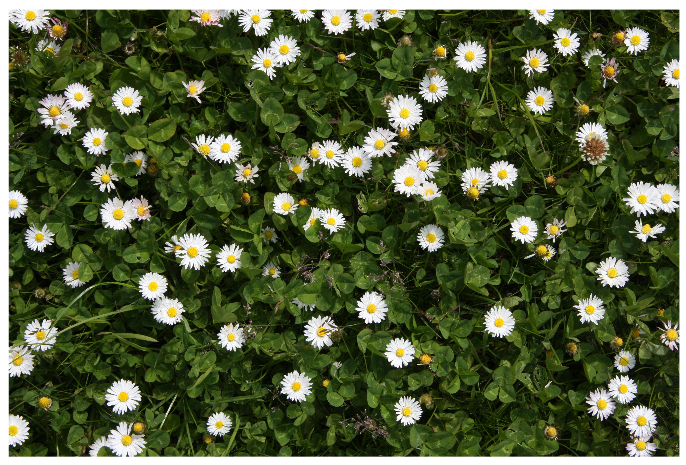
\includegraphics{flower.png}}
\efigure
\ecenter
\eblock

\end{frame}
%%%%%%%%%%%%%%%%%%%%%%%%%%%%%%%%%%%%%%%%%%%%%%%%%%%%%%%%%%%%%%%%%%%%
%%%%%%%%%%%%%%%%%%%%%%%%%%%%%%%%%%%%%%%%%%%%%%%%%%%%%%%%%%%%%%%
\begin{frame}
\frametitle{Complete Spatial Randomness (CSR)}

\bblock{Complete Spatial Randomness (CSR)}
\bitemize
\item yardstick, reference model that observed point patterns could be compared with, i.e., null hypothesis
\item = {\it homogeneous (uniform) Poisson point process} 
\item basic properties:
\bitemize
\item the number of points falling in any region $A$ has a Poisson distribution with mean $\lambda|A|$
\item given that there are $n$ points inside region $A$, the locations of these points are i.i.d. and uniformly distributed inside $A$
\item the contents of two disjoint regions $A$ and $B$ are independent 
\eitemize
\eitemize
\eblock
\bblock{Example:}
\vspace{-0.5cm}


{\centering \includegraphics[width=.3\linewidth]{figure/point-csr1} 
\includegraphics[width=.3\linewidth]{figure/point-csr2} 

}




\eblock

\end{frame}
%%%%%%%%%%%%%%%%%%%%%%%%%%%%%%%%%%%%%%%%%%%%%%%%%%%%%%%%%%%%%%%%%%%%

%%%%%%%%%%%%%%%%%%%%%%%%%%%%%%%%%%%%%%%%%%%%%%%%%%%%%%%%%%%%%%%
\begin{frame}
\frametitle{Quadrat counting test for CSR}

\bblock{Quadrat counting test}
\bitemize
\item partition study area $A$ into $L$ sub-regions (quadrats), $A_1, \ldots, A_L$ 
\item count number of events $n(A_l)$ in each sub-region $A_l$
\item Under the null hypothesis of CSR, the $n(A_l)$ are i.i.d. Poisson random variables with the same expected value
\item The Pearson $\chi^2$ goodness-of-fit test can be used 
\bitemize
\item test statistics: Pearson residual $\sum_{l}\epsilon(A_l)^2$
\[
\epsilon(A_l) = \frac{n(A_l) - \mu(A_l)}{\sqrt{{\mu(A_l)}}},
\]
where $\mu(A_l)$ indicates the expected number of events in $A_l$
\item $\sum_{l=1}\epsilon(A_l)^2$ is assumed to follow $\chi^2$ distribution
\eitemize
\eitemize
\eblock
\end{frame}
%%%%%%%%%%%%%%%%%%%%%%%%%%%%%%%%%%%%%%%%%%%%%%%%%%%%%%%%%%%%%%%%%%%%

%%%%%%%%%%%%%%%%%%%%%%%%%%%%%%%%%%%%%%%%%%%%%%%%%%%%%%%%%%%%%%%
\begin{frame}
\frametitle{Quadrat counting test for CSR}

\bblock{Example}
\vspace{-1cm}


{\centering \includegraphics[width=.3\linewidth]{figure/point-quadrattest} 

}




\bitemize
\item three values indicate the number of observations, CSR-expected number of observations, and the Pearson residuals 
\item $p$-value = $0.617$
\eitemize
\eblock
\end{frame}
%%%%%%%%%%%%%%%%%%%%%%%%%%%%%%%%%%%%%%%%%%%%%%%%%%%%%%%%%%%%%%%%%%%%

%%%%%%%%%%%%%%%%%%%%%%%%%%%%%%%%%%%%%%%%%%%%%%%%%%%%%%%%%%%%%%%
\begin{frame}
\frametitle{Nearest Neighbour Index (NNI) test under CSR}

\bblock{Nearest neighbour index}
\bitemize
\item Compares the mean of the distance observed between each point and its nearest neighbor ($\bar{d}_{min}$) and the expected mean distance under CSR $E(d_{min})$
\[
NNI=\frac{\bar{d}_{min}}{E(d_{min})}
\]
\item Under CSR, we have:
\[
E(d_{min})=\frac{1}{2\sqrt{\lambda}}
\]

\[
\sigma(d_{min})=\frac{0.26136}{\sqrt{{n^2}/{A}}}
\]
\eitemize
\eblock

\end{frame}
%%%%%%%%%%%%%%%%%%%%%%%%%%%%%%%%%%%%%%%%%%%%%%%%%%%%%%%%%%%%%%%%%%%%

%%%%%%%%%%%%%%%%%%%%%%%%%%%%%%%%%%%%%%%%%%%%%%%%%%%%%%%%%%%%%%%
\begin{frame}
\frametitle{Nearest Neighbour Index (NNI) test under CSR}


\bblock{Nearest neighbour index test}
\bitemize
\item Test statistics:
\[
z=\frac{\bar{d}_{min}-E(d_{min})}{\sigma(d_{min})},
\]
\item $z$ is assumed to follow Gaussian distribution, thus, if $z<-1,96$ or $z>1.96$, we are $95\%$ confident that the distribution is \underline {not} randomly distributed
\eitemize
\eblock
\end{frame}
%%%%%%%%%%%%%%%%%%%%%%%%%%%%%%%%%%%%%%%%%%%%%%%%%%%%%%%%%%%%%%%%%%%%

%%%%%%%%%%%%%%%%%%%%%%%%%%%%%%%%%%%%%%%%%%%%%%%%%%%%%%%%%%%%%%%
\begin{frame}
\frametitle{The G Function under CSR}

\bitemize
\item The G function is a function of nearest-neighbour distances
\item For a homogeneous Poisson point process of intensity $\lambda$, the nearest-neighour distance distribution (the G function) is known to be:
\[
G(d) = 1-\exp\{-\lambda\pi d^2\}
\]
\eitemize

\bblock{Example}
\begin{knitrout}
\definecolor{shadecolor}{rgb}{0.969, 0.969, 0.969}\color{fgcolor}

{\centering \includegraphics[width=.3\linewidth]{figure/point-gtest1} 
\includegraphics[width=.3\linewidth]{figure/point-gtest2} 

}



\end{knitrout}

\eblock

\end{frame}
%%%%%%%%%%%%%%%%%%%%%%%%%%%%%%%%%%%%%%%%%%%%%%%%%%%%%%%%%%%%%%%%%%%%

%%%%%%%%%%%%%%%%%%%%%%%%%%%%%%%%%%%%%%%%%%%%%%%%%%%%%%%%%%%%%%%
\begin{frame}
\frametitle{The F Function under CSR}

\bitemize
\item The F function is a function of empty space distances
\item For a homogeneous Poisson point process of intensity $\lambda$, the empty space distance distribution (the F function)is known to be:
\[
F(d) = 1-\exp\{-\lambda\pi d^2\}
\]
\item Equivalent to the G function 
\item Intuitively, because points (events) of the Poisson process are independent of each other, the knowledge that a random point is a 
event of a point pattern does not affect any other event of the process
\eitemize

\bblock{Example}
\begin{knitrout}
\definecolor{shadecolor}{rgb}{0.969, 0.969, 0.969}\color{fgcolor}

{\centering \includegraphics[width=.3\linewidth]{figure/point-Ftest1} 
\includegraphics[width=.3\linewidth]{figure/point-Ftest2} 

}



\end{knitrout}

\eblock

\end{frame}
%%%%%%%%%%%%%%%%%%%%%%%%%%%%%%%%%%%%%%%%%%%%%%%%%%%%%%%%%%%%%%%%%%%%

%%%%%%%%%%%%%%%%%%%%%%%%%%%%%%%%%%%%%%%%%%%%%%%%%%%%%%%%%%%%%%%
\begin{frame}
\frametitle{The K Function under CSR}

\bitemize
\item The K function is a function of pair-wise distances
\item For a homogeneous Poisson point process of intensity $\lambda$, the pair-wise distance distribution (the K function) is known to be:
\[
K(d) = \pi d^2\
\]
\item A commonly-used transformation of K is the L-function:
\[
L(d) = \sqrt{\frac{K(d)}{\pi}} = d
\]
\eitemize

\bblock{Example}
\begin{knitrout}
\definecolor{shadecolor}{rgb}{0.969, 0.969, 0.969}\color{fgcolor}

{\centering \includegraphics[width=.3\linewidth]{figure/point-Ktest1} 
\includegraphics[width=.3\linewidth]{figure/point-Ktest2} 
\includegraphics[width=.3\linewidth]{figure/point-Ktest3} 

}



\end{knitrout}

\eblock

\end{frame}
%%%%%%%%%%%%%%%%%%%%%%%%%%%%%%%%%%%%%%%%%%%%%%%%%%%%%%%%%%%%%%%%%%%%

%%%%%%%%%%%%%%%%%%%%%%%%%%%%%%%%%%%%%%%%%%%%%%%%%%%%%%%%%%%%%%%
\begin{frame}
\frametitle{Monte Carlo test}

\bitemize 
\item because of random variability, we will never obtain perfect
agreement between sample functions (say the K function) with theoretical
functions (the theoretical K functions), even with a completely random pattern
\eitemize

\bblock{Example}
\begin{knitrout}
\definecolor{shadecolor}{rgb}{0.969, 0.969, 0.969}\color{fgcolor}

{\centering \includegraphics[width=.3\linewidth]{figure/point-monte} 

}



\end{knitrout}

\eblock
\end{frame}
%%%%%%%%%%%%%%%%%%%%%%%%%%%%%%%%%%%%%%%%%%%%%%%%%%%%%%%%%%%%%%%%%%%%

%%%%%%%%%%%%%%%%%%%%%%%%%%%%%%%%%%%%%%%%%%%%%%%%%%%%%%%%%%%%%%%
\begin{frame}
\frametitle{Monte Carlo test}

\bitemize 
\item A {\it Monte Carlo} test is a test based on simulations from the null hypothesis 
\item Basic procedures:
\bitemize
\item generate $M$ independent simulations of CSR inside the study region $A$ 
\item compute the estimated K functions for each of these realisations, say $\hat{K}^{(j)}(r)$ for $j = 1, \ldots ,M$
\item obtain the pointwise upper and lower envelopes of these simulated curves
\item \underline{not} a confidence interval
\eitemize
\eitemize

\bblock{Example}
\begin{knitrout}
\definecolor{shadecolor}{rgb}{0.969, 0.969, 0.969}\color{fgcolor}

{\centering \includegraphics[width=.3\linewidth]{figure/point-monte2} 

}



\end{knitrout}


\eblock
\end{frame}
%%%%%%%%%%%%%%%%%%%%%%%%%%%%%%%%%%%%%%%%%%%%%%%%%%%%%%%%%%%%%%%%%%%%
%%%%%%%%%%%%%%%%%%%%%%%%%%%%%%%%%%%%%%%%%%%%%%%%%%%%%%%%%%%%%%%
\begin{frame}
\frametitle{Recap}

\bblock{Statitsical analysis of spatial point patterns:}
\bitemize
\item allows to quantify departure of results obtained via exploratory tools, e.g., $\hat{G}(d)$, from expected such results derived
under specific null hypotheses, here CSR hypothesis
\item can be used to assess to what extent observed point patterns can
be regarded as realizations from a particular spatial process (here CSR)
\item Same concepts can be applied for hypothesis of other types of point processes (e.g., Poisson cluster process, Cox process)
\eitemize
\eblock

\bblock{Sampling distribution of a test statistics}
\bitemize
\item lies at the heart of any statistical hypothesis testing procedure,
and is tied to a particular null hypothesis 
\item simulation and analytical derivations are two alternative ways of
computing such sampling distributions (the latter being increasingly replaced by the former)
\eitemize
\eblock

\bblock{Edge Effects}
\eblock

\end{frame}
%%%%%%%%%%%%%%%%%%%%%%%%%%%%%%%%%%%%%%%%%%%%%%%%%%%%%%%%%%%%%%%%%%%%

%%%%%%%%%%%%%%%%%%%%%%%%%%%%%%%%%%%%%%%%%%%%%%%%%%%%%%%%%%%%%%%%%%%%
%\begin{frame}
%\frametitle{Thanks}
%\bblock{Thank you, any questions?}
%\eblock
%\end{frame}
%%%%%%%%%%%%%%%%%%%%%%%%%%%%%%%%%%%%%%%%%%%%%%%%%%%%%%%%%%%%%%%%%%%%%
\end{document} 
